\documentclass[1p]{elsarticle_modified}
%\bibliographystyle{elsarticle-num}

%\usepackage[colorlinks]{hyperref}
%\usepackage{abbrmath_seonhwa} %\Abb, \Ascr, \Acal ,\Abf, \Afrak
\usepackage{amsfonts}
\usepackage{amssymb}
\usepackage{amsmath}
\usepackage{amsthm}
\usepackage{scalefnt}
\usepackage{amsbsy}
\usepackage{kotex}
\usepackage{caption}
\usepackage{subfig}
\usepackage{color}
\usepackage{graphicx}
\usepackage{xcolor} %% white, black, red, green, blue, cyan, magenta, yellow
\usepackage{float}
\usepackage{setspace}
\usepackage{hyperref}

\usepackage{tikz}
\usetikzlibrary{arrows}

\usepackage{multirow}
\usepackage{array} % fixed length table
\usepackage{hhline}

%%%%%%%%%%%%%%%%%%%%%
\makeatletter
\renewcommand*\env@matrix[1][\arraystretch]{%
	\edef\arraystretch{#1}%
	\hskip -\arraycolsep
	\let\@ifnextchar\new@ifnextchar
	\array{*\c@MaxMatrixCols c}}
\makeatother %https://tex.stackexchange.com/questions/14071/how-can-i-increase-the-line-spacing-in-a-matrix
%%%%%%%%%%%%%%%

\usepackage[normalem]{ulem}

\newcommand{\msout}[1]{\ifmmode\text{\sout{\ensuremath{#1}}}\else\sout{#1}\fi}
%SOURCE: \msout is \stkout macro in https://tex.stackexchange.com/questions/20609/strikeout-in-math-mode

\newcommand{\cancel}[1]{
	\ifmmode
	{\color{red}\msout{#1}}
	\else
	{\color{red}\sout{#1}}
	\fi
}

\newcommand{\add}[1]{
	{\color{blue}\uwave{#1}}
}

\newcommand{\replace}[2]{
	\ifmmode
	{\color{red}\msout{#1}}{\color{blue}\uwave{#2}}
	\else
	{\color{red}\sout{#1}}{\color{blue}\uwave{#2}}
	\fi
}

\newcommand{\Sol}{\mathcal{S}} %segment
\newcommand{\D}{D} %diagram
\newcommand{\A}{\mathcal{A}} %arc


%%%%%%%%%%%%%%%%%%%%%%%%%%%%%5 test

\def\sl{\operatorname{\textup{SL}}(2,\Cbb)}
\def\psl{\operatorname{\textup{PSL}}(2,\Cbb)}
\def\quan{\mkern 1mu \triangleright \mkern 1mu}

\theoremstyle{definition}
\newtheorem{thm}{Theorem}[section]
\newtheorem{prop}[thm]{Proposition}
\newtheorem{lem}[thm]{Lemma}
\newtheorem{ques}[thm]{Question}
\newtheorem{cor}[thm]{Corollary}
\newtheorem{defn}[thm]{Definition}
\newtheorem{exam}[thm]{Example}
\newtheorem{rmk}[thm]{Remark}
\newtheorem{alg}[thm]{Algorithm}

\newcommand{\I}{\sqrt{-1}}
\begin{document}

%\begin{frontmatter}
%
%\title{Boundary parabolic representations of knots up to 8 crossings}
%
%%% Group authors per affiliation:
%\author{Yunhi Cho} 
%\address{Department of Mathematics, University of Seoul, Seoul, Korea}
%\ead{yhcho@uos.ac.kr}
%
%
%\author{Seonhwa Kim} %\fnref{s_kim}}
%\address{Center for Geometry and Physics, Institute for Basic Science, Pohang, 37673, Korea}
%\ead{ryeona17@ibs.re.kr}
%
%\author{Hyuk Kim}
%\address{Department of Mathematical Sciences, Seoul National University, Seoul 08826, Korea}
%\ead{hyukkim@snu.ac.kr}
%
%\author{Seokbeom Yoon}
%\address{Department of Mathematical Sciences, Seoul National University, Seoul, 08826,  Korea}
%\ead{sbyoon15@snu.ac.kr}
%
%\begin{abstract}
%We find all boundary parabolic representation of knots up to 8 crossings.
%
%\end{abstract}
%\begin{keyword}
%    \MSC[2010] 57M25 
%\end{keyword}
%
%\end{frontmatter}

%\linenumbers
%\tableofcontents
%
\newcommand\colored[1]{\textcolor{white}{\rule[-0.35ex]{0.8em}{1.4ex}}\kern-0.8em\color{red} #1}%
%\newcommand\colored[1]{\textcolor{white}{ #1}\kern-2.17ex	\textcolor{white}{ #1}\kern-1.81ex	\textcolor{white}{ #1}\kern-2.15ex\color{red}#1	}

{\Large $\underline{12a_{0319}~(K12a_{0319})}$}

\setlength{\tabcolsep}{10pt}
\renewcommand{\arraystretch}{1.6}
\vspace{1cm}\begin{tabular}{m{100pt}>{\centering\arraybackslash}m{274pt}}
\multirow{5}{120pt}{
	\centering
	\includegraphics[width=112pt]{../../../GIT/diagram.site/Diagrams/png/1120_12a_0319.png}\\
\ \ \ A knot diagram\footnotemark}&
\allowdisplaybreaks
\textbf{Linearized knot diagam} \\
\cline{2-2}
 &
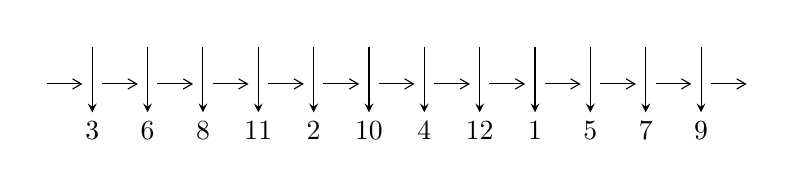
\begin{tikzpicture}[x=20pt, y=17pt]
	% nodes
	\node (C0) at (0, 0) {};
	\node (C1) at (1, 0) {};
	\node (C1U) at (1, +1) {};
	\node (C1D) at (1, -1) {3};

	\node (C2) at (2, 0) {};
	\node (C2U) at (2, +1) {};
	\node (C2D) at (2, -1) {6};

	\node (C3) at (3, 0) {};
	\node (C3U) at (3, +1) {};
	\node (C3D) at (3, -1) {8};

	\node (C4) at (4, 0) {};
	\node (C4U) at (4, +1) {};
	\node (C4D) at (4, -1) {11};

	\node (C5) at (5, 0) {};
	\node (C5U) at (5, +1) {};
	\node (C5D) at (5, -1) {2};

	\node (C6) at (6, 0) {};
	\node (C6U) at (6, +1) {};
	\node (C6D) at (6, -1) {10};

	\node (C7) at (7, 0) {};
	\node (C7U) at (7, +1) {};
	\node (C7D) at (7, -1) {4};

	\node (C8) at (8, 0) {};
	\node (C8U) at (8, +1) {};
	\node (C8D) at (8, -1) {12};

	\node (C9) at (9, 0) {};
	\node (C9U) at (9, +1) {};
	\node (C9D) at (9, -1) {1};

	\node (C10) at (10, 0) {};
	\node (C10U) at (10, +1) {};
	\node (C10D) at (10, -1) {5};

	\node (C11) at (11, 0) {};
	\node (C11U) at (11, +1) {};
	\node (C11D) at (11, -1) {7};

	\node (C12) at (12, 0) {};
	\node (C12U) at (12, +1) {};
	\node (C12D) at (12, -1) {9};
	\node (C13) at (13, 0) {};

	% arrows
	\draw[->,>={angle 60}]
	(C0) edge (C1) (C1) edge (C2) (C2) edge (C3) (C3) edge (C4) (C4) edge (C5) (C5) edge (C6) (C6) edge (C7) (C7) edge (C8) (C8) edge (C9) (C9) edge (C10) (C10) edge (C11) (C11) edge (C12) (C12) edge (C13) ;	\draw[->,>=stealth]
	(C1U) edge (C1D) (C2U) edge (C2D) (C3U) edge (C3D) (C4U) edge (C4D) (C5U) edge (C5D) (C6U) edge (C6D) (C7U) edge (C7D) (C8U) edge (C8D) (C9U) edge (C9D) (C10U) edge (C10D) (C11U) edge (C11D) (C12U) edge (C12D) ;
	\end{tikzpicture} \\
\hhline{~~} \\& 
\textbf{Solving Sequence} \\ \cline{2-2} 
 &
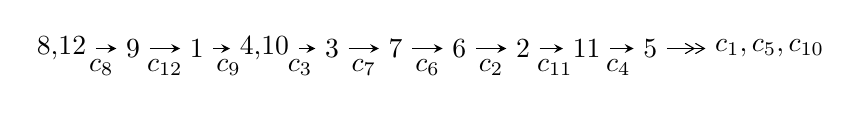
\begin{tikzpicture}[x=23pt, y=7pt]
	% node
	\node (A0) at (-1/8, 0) {8,12};
	\node (A1) at (1, 0) {9};
	\node (A2) at (2, 0) {1};
	\node (A3) at (49/16, 0) {4,10};
	\node (A4) at (33/8, 0) {3};
	\node (A5) at (41/8, 0) {7};
	\node (A6) at (49/8, 0) {6};
	\node (A7) at (57/8, 0) {2};
	\node (A8) at (65/8, 0) {11};
	\node (A9) at (73/8, 0) {5};
	\node (C1) at (1/2, -1) {$c_{8}$};
	\node (C2) at (3/2, -1) {$c_{12}$};
	\node (C3) at (5/2, -1) {$c_{9}$};
	\node (C4) at (29/8, -1) {$c_{3}$};
	\node (C5) at (37/8, -1) {$c_{7}$};
	\node (C6) at (45/8, -1) {$c_{6}$};
	\node (C7) at (53/8, -1) {$c_{2}$};
	\node (C8) at (61/8, -1) {$c_{11}$};
	\node (C9) at (69/8, -1) {$c_{4}$};
	\node (A10) at (11, 0) {$c_{1},c_{5},c_{10}$};

	% edge
	\draw[->,>=stealth]	
	(A0) edge (A1) (A1) edge (A2) (A2) edge (A3) (A3) edge (A4) (A4) edge (A5) (A5) edge (A6) (A6) edge (A7) (A7) edge (A8) (A8) edge (A9) ;
	\draw[->>,>={angle 60}]	
	(A9) edge (A10);
\end{tikzpicture} \\ 

\end{tabular} \\

\footnotetext{
The image of knot diagram is generated by the software ``\textbf{Draw programme}" developed by Andrew Bartholomew(\url{http://www.layer8.co.uk/maths/draw/index.htm\#Running-draw}), where we modified some parts for our purpose(\url{https://github.com/CATsTAILs/LinksPainter}).
}\phantom \\ \newline 
\centering \textbf{Ideals for irreducible components\footnotemark of $X_{\text{par}}$} 
 
\begin{align*}
I^u_{1}&=\langle 
3.23946\times10^{261} u^{112}-2.19296\times10^{262} u^{111}+\cdots+7.08037\times10^{259} b+1.92330\times10^{263},\\
\phantom{I^u_{1}}&\phantom{= \langle  }2.70622\times10^{262} u^{112}-1.87120\times10^{263} u^{111}+\cdots+5.16867\times10^{261} a+1.72060\times10^{264},\\
\phantom{I^u_{1}}&\phantom{= \langle  }u^{113}-8 u^{112}+\cdots-191 u-73\rangle \\
I^u_{2}&=\langle 
-9 u^{21}+23 u^{20}+\cdots+b+5,\;10 u^{21}-23 u^{20}+\cdots+a-8,\;u^{22}- u^{21}+\cdots-5 u-1\rangle \\
\\
\end{align*}
\raggedright * 2 irreducible components of $\dim_{\mathbb{C}}=0$, with total 135 representations.\\
\footnotetext{All coefficients of polynomials are rational numbers. But the coefficients are sometimes approximated in decimal forms when there is not enough margin.}
\newpage
\renewcommand{\arraystretch}{1}
\centering \section*{I. $I^u_{1}= \langle 3.24\times10^{261} u^{112}-2.19\times10^{262} u^{111}+\cdots+7.08\times10^{259} b+1.92\times10^{263},\;2.71\times10^{262} u^{112}-1.87\times10^{263} u^{111}+\cdots+5.17\times10^{261} a+1.72\times10^{264},\;u^{113}-8 u^{112}+\cdots-191 u-73 \rangle$}
\flushleft \textbf{(i) Arc colorings}\\
\begin{tabular}{m{7pt} m{180pt} m{7pt} m{180pt} }
\flushright $a_{8}=$&$\begin{pmatrix}1\\0\end{pmatrix}$ \\
\flushright $a_{12}=$&$\begin{pmatrix}0\\u\end{pmatrix}$ \\
\flushright $a_{9}=$&$\begin{pmatrix}1\\u^2\end{pmatrix}$ \\
\flushright $a_{1}=$&$\begin{pmatrix}- u\\- u^3+u\end{pmatrix}$ \\
\flushright $a_{4}=$&$\begin{pmatrix}-5.23581 u^{112}+36.2026 u^{111}+\cdots-1165.75 u-332.890\\-45.7527 u^{112}+309.724 u^{111}+\cdots-9315.33 u-2716.38\end{pmatrix}$ \\
\flushright $a_{10}=$&$\begin{pmatrix}- u^2+1\\- u^4+2 u^2\end{pmatrix}$ \\
\flushright $a_{3}=$&$\begin{pmatrix}-50.9886 u^{112}+345.927 u^{111}+\cdots-10481.1 u-3049.27\\-45.7527 u^{112}+309.724 u^{111}+\cdots-9315.33 u-2716.38\end{pmatrix}$ \\
\flushright $a_{7}=$&$\begin{pmatrix}22.5547 u^{112}-150.445 u^{111}+\cdots+4155.12 u+1233.81\\55.5418 u^{112}-373.123 u^{111}+\cdots+10722.4 u+3159.25\end{pmatrix}$ \\
\flushright $a_{6}=$&$\begin{pmatrix}53.6085 u^{112}-358.658 u^{111}+\cdots+10074.6 u+2982.05\\31.1098 u^{112}-209.344 u^{111}+\cdots+6063.36 u+1783.81\end{pmatrix}$ \\
\flushright $a_{2}=$&$\begin{pmatrix}49.0069 u^{112}-325.058 u^{111}+\cdots+8714.16 u+2609.75\\2.59511 u^{112}-18.1179 u^{111}+\cdots+624.353 u+175.782\end{pmatrix}$ \\
\flushright $a_{11}=$&$\begin{pmatrix}-3.49460 u^{112}+18.8084 u^{111}+\cdots+151.028 u+1.84444\\13.5515 u^{112}-89.8960 u^{111}+\cdots+2439.20 u+726.982\end{pmatrix}$ \\
\flushright $a_{5}=$&$\begin{pmatrix}47.0830 u^{112}-316.127 u^{111}+\cdots+9059.41 u+2671.49\\-22.4658 u^{112}+148.377 u^{111}+\cdots-3832.59 u-1156.94\end{pmatrix}$\\&\end{tabular}
\flushleft \textbf{(ii) Obstruction class $= -1$}\\~\\
\flushleft \textbf{(iii) Cusp Shapes $= 100.962 u^{112}-690.513 u^{111}+\cdots+21787.1 u+6280.51$}\\~\\
\newpage\renewcommand{\arraystretch}{1}
\flushleft \textbf{(iv) u-Polynomials at the component}\newline \\
\begin{tabular}{m{50pt}|m{274pt}}
Crossings & \hspace{64pt}u-Polynomials at each crossing \\
\hline $$\begin{aligned}c_{1}\end{aligned}$$&$\begin{aligned}
&u^{113}+47 u^{112}+\cdots+10403 u+169
\end{aligned}$\\
\hline $$\begin{aligned}c_{2},c_{5}\end{aligned}$$&$\begin{aligned}
&u^{113}+3 u^{112}+\cdots-69 u+13
\end{aligned}$\\
\hline $$\begin{aligned}c_{3},c_{7}\end{aligned}$$&$\begin{aligned}
&u^{113}+2 u^{112}+\cdots+12910 u+3551
\end{aligned}$\\
\hline $$\begin{aligned}c_{4},c_{10}\end{aligned}$$&$\begin{aligned}
&u^{113}- u^{112}+\cdots+14 u+1
\end{aligned}$\\
\hline $$\begin{aligned}c_{6}\end{aligned}$$&$\begin{aligned}
&u^{113}+8 u^{112}+\cdots-3489 u+907
\end{aligned}$\\
\hline $$\begin{aligned}c_{8},c_{9},c_{12}\end{aligned}$$&$\begin{aligned}
&u^{113}+8 u^{112}+\cdots-191 u+73
\end{aligned}$\\
\hline $$\begin{aligned}c_{11}\end{aligned}$$&$\begin{aligned}
&u^{113}-2 u^{112}+\cdots+277357 u+17593
\end{aligned}$\\
\hline
\end{tabular}\\~\\
\newpage\renewcommand{\arraystretch}{1}
\flushleft \textbf{(v) Riley Polynomials at the component}\newline \\
\begin{tabular}{m{50pt}|m{274pt}}
Crossings & \hspace{64pt}Riley Polynomials at each crossing \\
\hline $$\begin{aligned}c_{1}\end{aligned}$$&$\begin{aligned}
&y^{113}+49 y^{112}+\cdots+6847759 y-28561
\end{aligned}$\\
\hline $$\begin{aligned}c_{2},c_{5}\end{aligned}$$&$\begin{aligned}
&y^{113}-47 y^{112}+\cdots+10403 y-169
\end{aligned}$\\
\hline $$\begin{aligned}c_{3},c_{7}\end{aligned}$$&$\begin{aligned}
&y^{113}+80 y^{112}+\cdots+236395536 y-12609601
\end{aligned}$\\
\hline $$\begin{aligned}c_{4},c_{10}\end{aligned}$$&$\begin{aligned}
&y^{113}+95 y^{112}+\cdots-80 y-1
\end{aligned}$\\
\hline $$\begin{aligned}c_{6}\end{aligned}$$&$\begin{aligned}
&y^{113}+18 y^{112}+\cdots-6476613 y-822649
\end{aligned}$\\
\hline $$\begin{aligned}c_{8},c_{9},c_{12}\end{aligned}$$&$\begin{aligned}
&y^{113}-114 y^{112}+\cdots+78383 y-5329
\end{aligned}$\\
\hline $$\begin{aligned}c_{11}\end{aligned}$$&$\begin{aligned}
&y^{113}+26 y^{112}+\cdots-9594272227 y-309513649
\end{aligned}$\\
\hline
\end{tabular}\\~\\
\newpage\flushleft \textbf{(vi) Complex Volumes and Cusp Shapes}
$$\begin{array}{c|c|c}  
\text{Solutions to }I^u_{1}& \I (\text{vol} + \sqrt{-1}CS) & \text{Cusp shape}\\
 \hline 
\begin{aligned}
u &= \phantom{-}0.975525 + 0.343770 I \\
a &= -0.014156 - 0.379417 I \\
b &= -0.365622 + 0.526024 I\end{aligned}
 & -2.11411 + 1.42439 I & \phantom{-0.000000 } 0 \\ \hline\begin{aligned}
u &= \phantom{-}0.975525 - 0.343770 I \\
a &= -0.014156 + 0.379417 I \\
b &= -0.365622 - 0.526024 I\end{aligned}
 & -2.11411 - 1.42439 I & \phantom{-0.000000 } 0 \\ \hline\begin{aligned}
u &= -0.373774 + 0.872219 I \\
a &= -0.26773 - 1.92598 I \\
b &= -0.42020 + 1.35322 I\end{aligned}
 & \phantom{-}8.67189 + 7.43141 I & \phantom{-0.000000 } 0 \\ \hline\begin{aligned}
u &= -0.373774 - 0.872219 I \\
a &= -0.26773 + 1.92598 I \\
b &= -0.42020 - 1.35322 I\end{aligned}
 & \phantom{-}8.67189 - 7.43141 I & \phantom{-0.000000 } 0 \\ \hline\begin{aligned}
u &= -0.485419 + 0.943283 I \\
a &= \phantom{-}0.36391 + 1.70023 I \\
b &= \phantom{-}0.46917 - 1.37400 I\end{aligned}
 & \phantom{-}7.1075 + 13.2548 I & \phantom{-0.000000 } 0 \\ \hline\begin{aligned}
u &= -0.485419 - 0.943283 I \\
a &= \phantom{-}0.36391 - 1.70023 I \\
b &= \phantom{-}0.46917 + 1.37400 I\end{aligned}
 & \phantom{-}7.1075 - 13.2548 I & \phantom{-0.000000 } 0 \\ \hline\begin{aligned}
u &= \phantom{-}0.156511 + 0.903103 I \\
a &= -0.00785 - 1.68319 I \\
b &= \phantom{-}0.271493 + 1.096840 I\end{aligned}
 & \phantom{-}2.61440 - 2.49523 I & \phantom{-0.000000 } 0 \\ \hline\begin{aligned}
u &= \phantom{-}0.156511 - 0.903103 I \\
a &= -0.00785 + 1.68319 I \\
b &= \phantom{-}0.271493 - 1.096840 I\end{aligned}
 & \phantom{-}2.61440 + 2.49523 I & \phantom{-0.000000 } 0 \\ \hline\begin{aligned}
u &= \phantom{-}0.968058 + 0.543641 I \\
a &= -0.85420 + 1.31106 I \\
b &= -0.292289 - 0.886916 I\end{aligned}
 & -1.31892 - 1.43456 I & \phantom{-0.000000 } 0 \\ \hline\begin{aligned}
u &= \phantom{-}0.968058 - 0.543641 I \\
a &= -0.85420 - 1.31106 I \\
b &= -0.292289 + 0.886916 I\end{aligned}
 & -1.31892 + 1.43456 I & \phantom{-0.000000 } 0\\
 \hline 
 \end{array}$$\newpage$$\begin{array}{c|c|c}  
\text{Solutions to }I^u_{1}& \I (\text{vol} + \sqrt{-1}CS) & \text{Cusp shape}\\
 \hline 
\begin{aligned}
u &= -1.113700 + 0.087974 I \\
a &= \phantom{-}1.149820 + 0.422809 I \\
b &= \phantom{-}0.86338 - 1.17671 I\end{aligned}
 & \phantom{-}0.97417 + 5.88587 I & \phantom{-0.000000 } 0 \\ \hline\begin{aligned}
u &= -1.113700 - 0.087974 I \\
a &= \phantom{-}1.149820 - 0.422809 I \\
b &= \phantom{-}0.86338 + 1.17671 I\end{aligned}
 & \phantom{-}0.97417 - 5.88587 I & \phantom{-0.000000 } 0 \\ \hline\begin{aligned}
u &= \phantom{-}0.333656 + 1.095240 I \\
a &= -0.18854 + 1.49901 I \\
b &= -0.348286 - 1.040250 I\end{aligned}
 & \phantom{-}1.09765 - 7.03753 I & \phantom{-0.000000 } 0 \\ \hline\begin{aligned}
u &= \phantom{-}0.333656 - 1.095240 I \\
a &= -0.18854 - 1.49901 I \\
b &= -0.348286 + 1.040250 I\end{aligned}
 & \phantom{-}1.09765 + 7.03753 I & \phantom{-0.000000 } 0 \\ \hline\begin{aligned}
u &= -0.864544 + 0.773774 I \\
a &= \phantom{-}0.794215 + 1.007200 I \\
b &= -0.230925 - 1.207430 I\end{aligned}
 & \phantom{-}7.29213 - 1.91889 I & \phantom{-0.000000 } 0 \\ \hline\begin{aligned}
u &= -0.864544 - 0.773774 I \\
a &= \phantom{-}0.794215 - 1.007200 I \\
b &= -0.230925 + 1.207430 I\end{aligned}
 & \phantom{-}7.29213 + 1.91889 I & \phantom{-0.000000 } 0 \\ \hline\begin{aligned}
u &= -0.207224 + 0.808964 I \\
a &= -0.41108 - 1.57012 I \\
b &= \phantom{-}0.330697 + 1.230060 I\end{aligned}
 & \phantom{-}3.15474 - 2.44549 I & \phantom{-0.000000 } 0 \\ \hline\begin{aligned}
u &= -0.207224 - 0.808964 I \\
a &= -0.41108 + 1.57012 I \\
b &= \phantom{-}0.330697 - 1.230060 I\end{aligned}
 & \phantom{-}3.15474 + 2.44549 I & \phantom{-0.000000 } 0 \\ \hline\begin{aligned}
u &= \phantom{-}1.223500 + 0.011288 I \\
a &= -0.022574 + 0.318563 I \\
b &= -0.17684 - 2.01220 I\end{aligned}
 & \phantom{-}4.49179 - 3.00890 I & \phantom{-0.000000 } 0 \\ \hline\begin{aligned}
u &= \phantom{-}1.223500 - 0.011288 I \\
a &= -0.022574 - 0.318563 I \\
b &= -0.17684 + 2.01220 I\end{aligned}
 & \phantom{-}4.49179 + 3.00890 I & \phantom{-0.000000 } 0\\
 \hline 
 \end{array}$$\newpage$$\begin{array}{c|c|c}  
\text{Solutions to }I^u_{1}& \I (\text{vol} + \sqrt{-1}CS) & \text{Cusp shape}\\
 \hline 
\begin{aligned}
u &= -0.778711 + 0.951012 I \\
a &= -0.625337 - 1.042850 I \\
b &= \phantom{-}0.270860 + 1.248840 I\end{aligned}
 & \phantom{-}6.35326 - 7.05913 I & \phantom{-0.000000 } 0 \\ \hline\begin{aligned}
u &= -0.778711 - 0.951012 I \\
a &= -0.625337 + 1.042850 I \\
b &= \phantom{-}0.270860 - 1.248840 I\end{aligned}
 & \phantom{-}6.35326 + 7.05913 I & \phantom{-0.000000 } 0 \\ \hline\begin{aligned}
u &= -1.248140 + 0.059474 I \\
a &= \phantom{-}0.234772 + 1.097040 I \\
b &= \phantom{-}0.17298 - 1.50301 I\end{aligned}
 & \phantom{-}0.52000 + 3.23792 I & \phantom{-0.000000 } 0 \\ \hline\begin{aligned}
u &= -1.248140 - 0.059474 I \\
a &= \phantom{-}0.234772 - 1.097040 I \\
b &= \phantom{-}0.17298 + 1.50301 I\end{aligned}
 & \phantom{-}0.52000 - 3.23792 I & \phantom{-0.000000 } 0 \\ \hline\begin{aligned}
u &= \phantom{-}0.433114 + 0.608112 I \\
a &= \phantom{-}0.028879 - 0.629520 I \\
b &= -0.609339 + 0.178091 I\end{aligned}
 & -1.27678 - 3.46304 I & \phantom{-0.000000 } 0 \\ \hline\begin{aligned}
u &= \phantom{-}0.433114 - 0.608112 I \\
a &= \phantom{-}0.028879 + 0.629520 I \\
b &= -0.609339 - 0.178091 I\end{aligned}
 & -1.27678 + 3.46304 I & \phantom{-0.000000 } 0 \\ \hline\begin{aligned}
u &= \phantom{-}0.656590 + 0.313091 I \\
a &= -1.38222 + 1.74805 I \\
b &= -0.244826 - 0.839883 I\end{aligned}
 & -1.37943 - 1.39614 I & \phantom{-0.000000 } 0 \\ \hline\begin{aligned}
u &= \phantom{-}0.656590 - 0.313091 I \\
a &= -1.38222 - 1.74805 I \\
b &= -0.244826 + 0.839883 I\end{aligned}
 & -1.37943 + 1.39614 I & \phantom{-0.000000 } 0 \\ \hline\begin{aligned}
u &= -1.286140 + 0.038835 I \\
a &= -1.65307 + 1.17796 I \\
b &= -0.065458 - 0.916646 I\end{aligned}
 & -0.76391 + 6.11009 I & \phantom{-0.000000 } 0 \\ \hline\begin{aligned}
u &= -1.286140 - 0.038835 I \\
a &= -1.65307 - 1.17796 I \\
b &= -0.065458 + 0.916646 I\end{aligned}
 & -0.76391 - 6.11009 I & \phantom{-0.000000 } 0\\
 \hline 
 \end{array}$$\newpage$$\begin{array}{c|c|c}  
\text{Solutions to }I^u_{1}& \I (\text{vol} + \sqrt{-1}CS) & \text{Cusp shape}\\
 \hline 
\begin{aligned}
u &= \phantom{-}1.284900 + 0.078456 I \\
a &= -0.70832 + 2.15278 I \\
b &= -0.157497 - 1.404070 I\end{aligned}
 & \phantom{-}4.08065 - 4.21507 I & \phantom{-0.000000 } 0 \\ \hline\begin{aligned}
u &= \phantom{-}1.284900 - 0.078456 I \\
a &= -0.70832 - 2.15278 I \\
b &= -0.157497 + 1.404070 I\end{aligned}
 & \phantom{-}4.08065 + 4.21507 I & \phantom{-0.000000 } 0 \\ \hline\begin{aligned}
u &= \phantom{-}1.260290 + 0.295141 I \\
a &= -0.740145 + 0.650307 I \\
b &= -0.318857 - 1.008720 I\end{aligned}
 & -1.06984 - 1.80120 I & \phantom{-0.000000 } 0 \\ \hline\begin{aligned}
u &= \phantom{-}1.260290 - 0.295141 I \\
a &= -0.740145 - 0.650307 I \\
b &= -0.318857 + 1.008720 I\end{aligned}
 & -1.06984 + 1.80120 I & \phantom{-0.000000 } 0 \\ \hline\begin{aligned}
u &= \phantom{-}1.296470 + 0.038259 I \\
a &= \phantom{-}1.35156 + 0.46060 I \\
b &= \phantom{-}0.535281 - 0.867776 I\end{aligned}
 & -3.88087 - 1.65713 I & \phantom{-0.000000 } 0 \\ \hline\begin{aligned}
u &= \phantom{-}1.296470 - 0.038259 I \\
a &= \phantom{-}1.35156 - 0.46060 I \\
b &= \phantom{-}0.535281 + 0.867776 I\end{aligned}
 & -3.88087 + 1.65713 I & \phantom{-0.000000 } 0 \\ \hline\begin{aligned}
u &= -1.307720 + 0.013959 I \\
a &= -0.972701 + 0.271024 I \\
b &= -1.01921 - 1.20757 I\end{aligned}
 & \phantom{-}0.89650 - 2.18592 I & \phantom{-0.000000 } 0 \\ \hline\begin{aligned}
u &= -1.307720 - 0.013959 I \\
a &= -0.972701 - 0.271024 I \\
b &= -1.01921 + 1.20757 I\end{aligned}
 & \phantom{-}0.89650 + 2.18592 I & \phantom{-0.000000 } 0 \\ \hline\begin{aligned}
u &= \phantom{-}1.290090 + 0.230697 I \\
a &= -0.979250 + 0.508289 I \\
b &= -0.427447 - 0.996014 I\end{aligned}
 & -1.12305 - 1.91262 I & \phantom{-0.000000 } 0 \\ \hline\begin{aligned}
u &= \phantom{-}1.290090 - 0.230697 I \\
a &= -0.979250 - 0.508289 I \\
b &= -0.427447 + 0.996014 I\end{aligned}
 & -1.12305 + 1.91262 I & \phantom{-0.000000 } 0\\
 \hline 
 \end{array}$$\newpage$$\begin{array}{c|c|c}  
\text{Solutions to }I^u_{1}& \I (\text{vol} + \sqrt{-1}CS) & \text{Cusp shape}\\
 \hline 
\begin{aligned}
u &= -1.305330 + 0.149159 I \\
a &= \phantom{-}1.78259 + 0.55086 I \\
b &= \phantom{-}0.010684 - 0.999271 I\end{aligned}
 & \phantom{-}3.25522 + 0.04146 I & \phantom{-0.000000 } 0 \\ \hline\begin{aligned}
u &= -1.305330 - 0.149159 I \\
a &= \phantom{-}1.78259 - 0.55086 I \\
b &= \phantom{-}0.010684 + 0.999271 I\end{aligned}
 & \phantom{-}3.25522 - 0.04146 I & \phantom{-0.000000 } 0 \\ \hline\begin{aligned}
u &= -0.347724 + 0.586819 I \\
a &= -0.333304 + 0.035629 I \\
b &= \phantom{-}1.122950 - 0.208901 I\end{aligned}
 & \phantom{-}2.20924 + 7.86227 I & \phantom{-0.000000 } 0 \\ \hline\begin{aligned}
u &= -0.347724 - 0.586819 I \\
a &= -0.333304 - 0.035629 I \\
b &= \phantom{-}1.122950 + 0.208901 I\end{aligned}
 & \phantom{-}2.20924 - 7.86227 I & \phantom{-0.000000 } 0 \\ \hline\begin{aligned}
u &= \phantom{-}0.247843 + 0.629558 I \\
a &= \phantom{-}0.25253 - 1.62717 I \\
b &= \phantom{-}0.48616 + 1.53859 I\end{aligned}
 & \phantom{-}6.58164 + 0.99842 I & -12.00000 + 0. I\phantom{ +0.000000I} \\ \hline\begin{aligned}
u &= \phantom{-}0.247843 - 0.629558 I \\
a &= \phantom{-}0.25253 + 1.62717 I \\
b &= \phantom{-}0.48616 - 1.53859 I\end{aligned}
 & \phantom{-}6.58164 - 0.99842 I & -12.00000 + 0. I\phantom{ +0.000000I} \\ \hline\begin{aligned}
u &= \phantom{-}0.437621 + 0.466675 I \\
a &= -2.33498 + 0.42775 I \\
b &= \phantom{-}0.041597 - 1.270910 I\end{aligned}
 & \phantom{-}5.73774 - 4.28699 I & -7.05414 + 7.47196 I \\ \hline\begin{aligned}
u &= \phantom{-}0.437621 - 0.466675 I \\
a &= -2.33498 - 0.42775 I \\
b &= \phantom{-}0.041597 + 1.270910 I\end{aligned}
 & \phantom{-}5.73774 + 4.28699 I & -7.05414 - 7.47196 I \\ \hline\begin{aligned}
u &= -0.487973 + 0.412211 I \\
a &= -0.077880 + 0.628379 I \\
b &= \phantom{-}0.859901 + 0.154819 I\end{aligned}
 & -1.41996 + 1.43991 I & -14.1213 - 4.7302 I \\ \hline\begin{aligned}
u &= -0.487973 - 0.412211 I \\
a &= -0.077880 - 0.628379 I \\
b &= \phantom{-}0.859901 - 0.154819 I\end{aligned}
 & -1.41996 - 1.43991 I & -14.1213 + 4.7302 I\\
 \hline 
 \end{array}$$\newpage$$\begin{array}{c|c|c}  
\text{Solutions to }I^u_{1}& \I (\text{vol} + \sqrt{-1}CS) & \text{Cusp shape}\\
 \hline 
\begin{aligned}
u &= \phantom{-}1.369370 + 0.020352 I \\
a &= -0.172640 - 0.430954 I \\
b &= -0.543471 + 0.516438 I\end{aligned}
 & -1.93217 + 1.98337 I & \phantom{-0.000000 } 0 \\ \hline\begin{aligned}
u &= \phantom{-}1.369370 - 0.020352 I \\
a &= -0.172640 + 0.430954 I \\
b &= -0.543471 - 0.516438 I\end{aligned}
 & -1.93217 - 1.98337 I & \phantom{-0.000000 } 0 \\ \hline\begin{aligned}
u &= -0.474494 + 0.403935 I \\
a &= \phantom{-}1.86778 + 2.26063 I \\
b &= \phantom{-}0.458372 - 1.138950 I\end{aligned}
 & \phantom{-}1.58848 + 6.19220 I & -12.6737 - 8.9348 I \\ \hline\begin{aligned}
u &= -0.474494 - 0.403935 I \\
a &= \phantom{-}1.86778 - 2.26063 I \\
b &= \phantom{-}0.458372 + 1.138950 I\end{aligned}
 & \phantom{-}1.58848 - 6.19220 I & -12.6737 + 8.9348 I \\ \hline\begin{aligned}
u &= -0.374258 + 0.493118 I \\
a &= \phantom{-}0.95129 - 1.21092 I \\
b &= -0.378161 + 0.034177 I\end{aligned}
 & \phantom{-}3.77539 + 0.34718 I & -7.42485 - 3.96458 I \\ \hline\begin{aligned}
u &= -0.374258 - 0.493118 I \\
a &= \phantom{-}0.95129 + 1.21092 I \\
b &= -0.378161 - 0.034177 I\end{aligned}
 & \phantom{-}3.77539 - 0.34718 I & -7.42485 + 3.96458 I \\ \hline\begin{aligned}
u &= -0.159935 + 0.594286 I \\
a &= -0.93341 - 1.71005 I \\
b &= -0.079665 + 1.194920 I\end{aligned}
 & \phantom{-}3.39551 - 1.15967 I & -5.79218 + 3.05199 I \\ \hline\begin{aligned}
u &= -0.159935 - 0.594286 I \\
a &= -0.93341 + 1.71005 I \\
b &= -0.079665 - 1.194920 I\end{aligned}
 & \phantom{-}3.39551 + 1.15967 I & -5.79218 - 3.05199 I \\ \hline\begin{aligned}
u &= -1.373130 + 0.259161 I \\
a &= \phantom{-}0.831528 + 0.432014 I \\
b &= \phantom{-}0.95042 - 1.39994 I\end{aligned}
 & \phantom{-}1.45927 + 2.27600 I & \phantom{-0.000000 } 0 \\ \hline\begin{aligned}
u &= -1.373130 - 0.259161 I \\
a &= \phantom{-}0.831528 - 0.432014 I \\
b &= \phantom{-}0.95042 + 1.39994 I\end{aligned}
 & \phantom{-}1.45927 - 2.27600 I & \phantom{-0.000000 } 0\\
 \hline 
 \end{array}$$\newpage$$\begin{array}{c|c|c}  
\text{Solutions to }I^u_{1}& \I (\text{vol} + \sqrt{-1}CS) & \text{Cusp shape}\\
 \hline 
\begin{aligned}
u &= -1.404600 + 0.140162 I \\
a &= \phantom{-}0.260271 + 0.025626 I \\
b &= \phantom{-}1.005960 + 0.221517 I\end{aligned}
 & -5.62291 + 1.41549 I & \phantom{-0.000000 } 0 \\ \hline\begin{aligned}
u &= -1.404600 - 0.140162 I \\
a &= \phantom{-}0.260271 - 0.025626 I \\
b &= \phantom{-}1.005960 - 0.221517 I\end{aligned}
 & -5.62291 - 1.41549 I & \phantom{-0.000000 } 0 \\ \hline\begin{aligned}
u &= -0.383749 + 0.445783 I \\
a &= \phantom{-}1.38035 + 1.04092 I \\
b &= \phantom{-}0.335426 - 1.162020 I\end{aligned}
 & \phantom{-}2.45026 + 3.90445 I & -6.44576 - 2.61691 I \\ \hline\begin{aligned}
u &= -0.383749 - 0.445783 I \\
a &= \phantom{-}1.38035 - 1.04092 I \\
b &= \phantom{-}0.335426 + 1.162020 I\end{aligned}
 & \phantom{-}2.45026 - 3.90445 I & -6.44576 + 2.61691 I \\ \hline\begin{aligned}
u &= -0.239713 + 0.535309 I \\
a &= -1.22212 + 1.64034 I \\
b &= \phantom{-}0.213848 + 0.120182 I\end{aligned}
 & \phantom{-}2.18768 - 4.74508 I & -10.37642 + 0.76774 I \\ \hline\begin{aligned}
u &= -0.239713 - 0.535309 I \\
a &= -1.22212 - 1.64034 I \\
b &= \phantom{-}0.213848 - 0.120182 I\end{aligned}
 & \phantom{-}2.18768 + 4.74508 I & -10.37642 - 0.76774 I \\ \hline\begin{aligned}
u &= -0.337117 + 0.471029 I \\
a &= \phantom{-}0.661155 - 0.131613 I \\
b &= -0.928411 + 0.301402 I\end{aligned}
 & \phantom{-}3.71740 + 2.72095 I & -7.71498 - 4.87286 I \\ \hline\begin{aligned}
u &= -0.337117 - 0.471029 I \\
a &= \phantom{-}0.661155 + 0.131613 I \\
b &= -0.928411 - 0.301402 I\end{aligned}
 & \phantom{-}3.71740 - 2.72095 I & -7.71498 + 4.87286 I \\ \hline\begin{aligned}
u &= \phantom{-}1.41197 + 0.18152 I \\
a &= -0.346112 + 0.294720 I \\
b &= -1.352470 - 0.058009 I\end{aligned}
 & -1.83782 - 5.16732 I & \phantom{-0.000000 } 0 \\ \hline\begin{aligned}
u &= \phantom{-}1.41197 - 0.18152 I \\
a &= -0.346112 - 0.294720 I \\
b &= -1.352470 + 0.058009 I\end{aligned}
 & -1.83782 + 5.16732 I & \phantom{-0.000000 } 0\\
 \hline 
 \end{array}$$\newpage$$\begin{array}{c|c|c}  
\text{Solutions to }I^u_{1}& \I (\text{vol} + \sqrt{-1}CS) & \text{Cusp shape}\\
 \hline 
\begin{aligned}
u &= -1.44030 + 0.16888 I \\
a &= -0.836059 - 0.359382 I \\
b &= -1.02401 + 1.36719 I\end{aligned}
 & \phantom{-}1.25755 + 6.47322 I & \phantom{-0.000000 } 0 \\ \hline\begin{aligned}
u &= -1.44030 - 0.16888 I \\
a &= -0.836059 + 0.359382 I \\
b &= -1.02401 - 1.36719 I\end{aligned}
 & \phantom{-}1.25755 - 6.47322 I & \phantom{-0.000000 } 0 \\ \hline\begin{aligned}
u &= \phantom{-}1.44234 + 0.22727 I \\
a &= \phantom{-}0.370654 - 0.260708 I \\
b &= \phantom{-}1.45383 - 0.10554 I\end{aligned}
 & -3.56727 - 10.87880 I & \phantom{-0.000000 } 0 \\ \hline\begin{aligned}
u &= \phantom{-}1.44234 - 0.22727 I \\
a &= \phantom{-}0.370654 + 0.260708 I \\
b &= \phantom{-}1.45383 + 0.10554 I\end{aligned}
 & -3.56727 + 10.87880 I & \phantom{-0.000000 } 0 \\ \hline\begin{aligned}
u &= -1.42088 + 0.34291 I \\
a &= \phantom{-}0.810308 + 1.010290 I \\
b &= \phantom{-}0.549077 - 1.209210 I\end{aligned}
 & -2.53431 + 6.92079 I & \phantom{-0.000000 } 0 \\ \hline\begin{aligned}
u &= -1.42088 - 0.34291 I \\
a &= \phantom{-}0.810308 - 1.010290 I \\
b &= \phantom{-}0.549077 + 1.209210 I\end{aligned}
 & -2.53431 - 6.92079 I & \phantom{-0.000000 } 0 \\ \hline\begin{aligned}
u &= \phantom{-}1.45964 + 0.18053 I \\
a &= \phantom{-}1.041130 - 0.183211 I \\
b &= \phantom{-}0.569702 + 0.993657 I\end{aligned}
 & -3.55249 - 6.29900 I & \phantom{-0.000000 } 0 \\ \hline\begin{aligned}
u &= \phantom{-}1.45964 - 0.18053 I \\
a &= \phantom{-}1.041130 + 0.183211 I \\
b &= \phantom{-}0.569702 - 0.993657 I\end{aligned}
 & -3.55249 + 6.29900 I & \phantom{-0.000000 } 0 \\ \hline\begin{aligned}
u &= \phantom{-}1.46531 + 0.18133 I \\
a &= \phantom{-}1.30433 - 1.03874 I \\
b &= \phantom{-}0.507458 + 1.266340 I\end{aligned}
 & -4.63950 - 8.54288 I & \phantom{-0.000000 } 0 \\ \hline\begin{aligned}
u &= \phantom{-}1.46531 - 0.18133 I \\
a &= \phantom{-}1.30433 + 1.03874 I \\
b &= \phantom{-}0.507458 - 1.266340 I\end{aligned}
 & -4.63950 + 8.54288 I & \phantom{-0.000000 } 0\\
 \hline 
 \end{array}$$\newpage$$\begin{array}{c|c|c}  
\text{Solutions to }I^u_{1}& \I (\text{vol} + \sqrt{-1}CS) & \text{Cusp shape}\\
 \hline 
\begin{aligned}
u &= -1.46819 + 0.18027 I \\
a &= -1.45890 + 0.23517 I \\
b &= -0.070028 + 1.011290 I\end{aligned}
 & -0.43130 + 6.73555 I & \phantom{-0.000000 } 0 \\ \hline\begin{aligned}
u &= -1.46819 - 0.18027 I \\
a &= -1.45890 - 0.23517 I \\
b &= -0.070028 - 1.011290 I\end{aligned}
 & -0.43130 - 6.73555 I & \phantom{-0.000000 } 0 \\ \hline\begin{aligned}
u &= \phantom{-}0.289781 + 0.429902 I \\
a &= -0.64968 + 1.76717 I \\
b &= -0.62464 - 1.51753 I\end{aligned}
 & \phantom{-}6.92171 - 4.22400 I & -4.15858 + 8.77688 I \\ \hline\begin{aligned}
u &= \phantom{-}0.289781 - 0.429902 I \\
a &= -0.64968 - 1.76717 I \\
b &= -0.62464 + 1.51753 I\end{aligned}
 & \phantom{-}6.92171 + 4.22400 I & -4.15858 - 8.77688 I \\ \hline\begin{aligned}
u &= -1.46562 + 0.23557 I \\
a &= -0.259206 - 0.035445 I \\
b &= -0.992562 - 0.369481 I\end{aligned}
 & -7.38904 + 6.61296 I & \phantom{-0.000000 } 0 \\ \hline\begin{aligned}
u &= -1.46562 - 0.23557 I \\
a &= -0.259206 + 0.035445 I \\
b &= -0.992562 + 0.369481 I\end{aligned}
 & -7.38904 - 6.61296 I & \phantom{-0.000000 } 0 \\ \hline\begin{aligned}
u &= -1.47432 + 0.19366 I \\
a &= -0.846841 - 1.117710 I \\
b &= -0.440021 + 1.145260 I\end{aligned}
 & -7.94835 + 3.87685 I & \phantom{-0.000000 } 0 \\ \hline\begin{aligned}
u &= -1.47432 - 0.19366 I \\
a &= -0.846841 + 1.117710 I \\
b &= -0.440021 - 1.145260 I\end{aligned}
 & -7.94835 - 3.87685 I & \phantom{-0.000000 } 0 \\ \hline\begin{aligned}
u &= \phantom{-}0.095068 + 0.501846 I \\
a &= \phantom{-}2.34187 - 3.16314 I \\
b &= -0.175916 + 1.238840 I\end{aligned}
 & \phantom{-}7.57611 + 2.36095 I & \phantom{-}1.28578 - 1.07524 I \\ \hline\begin{aligned}
u &= \phantom{-}0.095068 - 0.501846 I \\
a &= \phantom{-}2.34187 + 3.16314 I \\
b &= -0.175916 - 1.238840 I\end{aligned}
 & \phantom{-}7.57611 - 2.36095 I & \phantom{-}1.28578 + 1.07524 I\\
 \hline 
 \end{array}$$\newpage$$\begin{array}{c|c|c}  
\text{Solutions to }I^u_{1}& \I (\text{vol} + \sqrt{-1}CS) & \text{Cusp shape}\\
 \hline 
\begin{aligned}
u &= \phantom{-}1.49752 + 0.09934 I \\
a &= \phantom{-}0.460213 - 0.381643 I \\
b &= \phantom{-}0.979596 - 0.220843 I\end{aligned}
 & -8.01183 - 3.20810 I & \phantom{-0.000000 } 0 \\ \hline\begin{aligned}
u &= \phantom{-}1.49752 - 0.09934 I \\
a &= \phantom{-}0.460213 + 0.381643 I \\
b &= \phantom{-}0.979596 + 0.220843 I\end{aligned}
 & -8.01183 + 3.20810 I & \phantom{-0.000000 } 0 \\ \hline\begin{aligned}
u &= \phantom{-}1.46984 + 0.32887 I \\
a &= -0.964403 + 1.011600 I \\
b &= -0.59155 - 1.41586 I\end{aligned}
 & \phantom{-}2.76721 - 11.75190 I & \phantom{-0.000000 } 0 \\ \hline\begin{aligned}
u &= \phantom{-}1.46984 - 0.32887 I \\
a &= -0.964403 - 1.011600 I \\
b &= -0.59155 + 1.41586 I\end{aligned}
 & \phantom{-}2.76721 + 11.75190 I & \phantom{-0.000000 } 0 \\ \hline\begin{aligned}
u &= \phantom{-}1.40529 + 0.63509 I \\
a &= \phantom{-}0.530354 - 1.153880 I \\
b &= \phantom{-}0.244714 + 0.870612 I\end{aligned}
 & -2.54902 - 4.87687 I & \phantom{-0.000000 } 0 \\ \hline\begin{aligned}
u &= \phantom{-}1.40529 - 0.63509 I \\
a &= \phantom{-}0.530354 + 1.153880 I \\
b &= \phantom{-}0.244714 - 0.870612 I\end{aligned}
 & -2.54902 + 4.87687 I & \phantom{-0.000000 } 0 \\ \hline\begin{aligned}
u &= -1.50400 + 0.39257 I \\
a &= -0.839195 - 0.995514 I \\
b &= -0.583955 + 1.164530 I\end{aligned}
 & -4.85144 + 12.24700 I & \phantom{-0.000000 } 0 \\ \hline\begin{aligned}
u &= -1.50400 - 0.39257 I \\
a &= -0.839195 + 0.995514 I \\
b &= -0.583955 - 1.164530 I\end{aligned}
 & -4.85144 - 12.24700 I & \phantom{-0.000000 } 0 \\ \hline\begin{aligned}
u &= \phantom{-}1.54260 + 0.27953 I \\
a &= \phantom{-}0.290487 - 0.954752 I \\
b &= \phantom{-}0.140916 + 0.940361 I\end{aligned}
 & -3.00503 + 1.08144 I & \phantom{-0.000000 } 0 \\ \hline\begin{aligned}
u &= \phantom{-}1.54260 - 0.27953 I \\
a &= \phantom{-}0.290487 + 0.954752 I \\
b &= \phantom{-}0.140916 - 0.940361 I\end{aligned}
 & -3.00503 - 1.08144 I & \phantom{-0.000000 } 0\\
 \hline 
 \end{array}$$\newpage$$\begin{array}{c|c|c}  
\text{Solutions to }I^u_{1}& \I (\text{vol} + \sqrt{-1}CS) & \text{Cusp shape}\\
 \hline 
\begin{aligned}
u &= \phantom{-}1.52947 + 0.35191 I \\
a &= \phantom{-}0.945790 - 0.924476 I \\
b &= \phantom{-}0.64869 + 1.40966 I\end{aligned}
 & \phantom{-}0.6370 - 17.9551 I & \phantom{-0.000000 } 0 \\ \hline\begin{aligned}
u &= \phantom{-}1.52947 - 0.35191 I \\
a &= \phantom{-}0.945790 + 0.924476 I \\
b &= \phantom{-}0.64869 - 1.40966 I\end{aligned}
 & \phantom{-}0.6370 + 17.9551 I & \phantom{-0.000000 } 0 \\ \hline\begin{aligned}
u &= \phantom{-}0.116869 + 0.408252 I \\
a &= -0.182161 + 1.077640 I \\
b &= \phantom{-}0.532481 + 0.072693 I\end{aligned}
 & -0.543296 + 0.399156 I & -13.17949 + 1.12118 I \\ \hline\begin{aligned}
u &= \phantom{-}0.116869 - 0.408252 I \\
a &= -0.182161 - 1.077640 I \\
b &= \phantom{-}0.532481 - 0.072693 I\end{aligned}
 & -0.543296 - 0.399156 I & -13.17949 - 1.12118 I \\ \hline\begin{aligned}
u &= \phantom{-}1.57011 + 0.25302 I \\
a &= \phantom{-}0.050722 + 0.414703 I \\
b &= \phantom{-}0.270653 - 0.751807 I\end{aligned}
 & -2.83313 - 2.36688 I & \phantom{-0.000000 } 0 \\ \hline\begin{aligned}
u &= \phantom{-}1.57011 - 0.25302 I \\
a &= \phantom{-}0.050722 - 0.414703 I \\
b &= \phantom{-}0.270653 + 0.751807 I\end{aligned}
 & -2.83313 + 2.36688 I & \phantom{-0.000000 } 0 \\ \hline\begin{aligned}
u &= -1.60463 + 0.04728 I \\
a &= -0.193464 - 0.069815 I \\
b &= -0.497661 - 0.282158 I\end{aligned}
 & -10.67240 - 0.12814 I & \phantom{-0.000000 } 0 \\ \hline\begin{aligned}
u &= -1.60463 - 0.04728 I \\
a &= -0.193464 + 0.069815 I \\
b &= -0.497661 + 0.282158 I\end{aligned}
 & -10.67240 + 0.12814 I & \phantom{-0.000000 } 0 \\ \hline\begin{aligned}
u &= -0.330981 + 0.091771 I \\
a &= \phantom{-}2.26299 + 1.65780 I \\
b &= -0.556933 - 0.972649 I\end{aligned}
 & \phantom{-}4.26850 - 2.16570 I & -14.8529 + 5.8248 I \\ \hline\begin{aligned}
u &= -0.330981 - 0.091771 I \\
a &= \phantom{-}2.26299 - 1.65780 I \\
b &= -0.556933 + 0.972649 I\end{aligned}
 & \phantom{-}4.26850 + 2.16570 I & -14.8529 - 5.8248 I\\
 \hline 
 \end{array}$$\newpage$$\begin{array}{c|c|c}  
\text{Solutions to }I^u_{1}& \I (\text{vol} + \sqrt{-1}CS) & \text{Cusp shape}\\
 \hline 
\begin{aligned}
u &= \phantom{-}0.295478\phantom{ +0.000000I} \\
a &= -0.892558\phantom{ +0.000000I} \\
b &= \phantom{-}0.325774\phantom{ +0.000000I}\end{aligned}
 & -0.572509\phantom{ +0.000000I} & -17.2100\phantom{ +0.000000I} \\ \hline\begin{aligned}
u &= \phantom{-}1.88523 + 0.07373 I \\
a &= \phantom{-}0.008429 + 0.394780 I \\
b &= \phantom{-}0.057063 - 0.952589 I\end{aligned}
 & -3.21447 + 1.94404 I & \phantom{-0.000000 } 0 \\ \hline\begin{aligned}
u &= \phantom{-}1.88523 - 0.07373 I \\
a &= \phantom{-}0.008429 - 0.394780 I \\
b &= \phantom{-}0.057063 + 0.952589 I\end{aligned}
 & -3.21447 - 1.94404 I & \phantom{-0.000000 } 0\\
 \hline 
 \end{array}$$\newpage\newpage\renewcommand{\arraystretch}{1}
\centering \section*{II. $I^u_{2}= \langle -9 u^{21}+23 u^{20}+\cdots+b+5,\;10 u^{21}-23 u^{20}+\cdots+a-8,\;u^{22}- u^{21}+\cdots-5 u-1 \rangle$}
\flushleft \textbf{(i) Arc colorings}\\
\begin{tabular}{m{7pt} m{180pt} m{7pt} m{180pt} }
\flushright $a_{8}=$&$\begin{pmatrix}1\\0\end{pmatrix}$ \\
\flushright $a_{12}=$&$\begin{pmatrix}0\\u\end{pmatrix}$ \\
\flushright $a_{9}=$&$\begin{pmatrix}1\\u^2\end{pmatrix}$ \\
\flushright $a_{1}=$&$\begin{pmatrix}- u\\- u^3+u\end{pmatrix}$ \\
\flushright $a_{4}=$&$\begin{pmatrix}-10 u^{21}+23 u^{20}+\cdots+38 u+8\\9 u^{21}-23 u^{20}+\cdots-27 u-5\end{pmatrix}$ \\
\flushright $a_{10}=$&$\begin{pmatrix}- u^2+1\\- u^4+2 u^2\end{pmatrix}$ \\
\flushright $a_{3}=$&$\begin{pmatrix}- u^{21}+17 u^{19}+\cdots+11 u+3\\9 u^{21}-23 u^{20}+\cdots-27 u-5\end{pmatrix}$ \\
\flushright $a_{7}=$&$\begin{pmatrix}-5 u^{21}+9 u^{20}+\cdots+27 u+10\\-3 u^{21}+6 u^{20}+\cdots+6 u+3\end{pmatrix}$ \\
\flushright $a_{6}=$&$\begin{pmatrix}-5 u^{21}+9 u^{20}+\cdots+25 u+10\\-2 u^{21}+4 u^{20}+\cdots+2 u+2\end{pmatrix}$ \\
\flushright $a_{2}=$&$\begin{pmatrix}14 u^{21}-31 u^{20}+\cdots-54 u-17\\- u^{21}+3 u^{20}+\cdots- u-2\end{pmatrix}$ \\
\flushright $a_{11}=$&$\begin{pmatrix}-10 u^{21}+28 u^{20}+\cdots+36 u^2+19 u\\3 u^{21}-7 u^{20}+\cdots-9 u-5\end{pmatrix}$ \\
\flushright $a_{5}=$&$\begin{pmatrix}5 u^{21}-9 u^{20}+\cdots-22 u-4\\-16 u^{21}+38 u^{20}+\cdots+41 u+8\end{pmatrix}$\\&\end{tabular}
\flushleft \textbf{(ii) Obstruction class $= 1$}\\~\\
\flushleft \textbf{(iii) Cusp Shapes $= 3 u^{21}-10 u^{20}-27 u^{19}+118 u^{18}+77 u^{17}-585 u^{16}+9 u^{15}+1570 u^{14}-503 u^{13}-2443 u^{12}+1076 u^{11}+2194 u^{10}-810 u^9-1096 u^8-74 u^7+324 u^6+327 u^5-51 u^4-49 u^3-42 u^2-11 u-5$}\\~\\
\newpage\renewcommand{\arraystretch}{1}
\flushleft \textbf{(iv) u-Polynomials at the component}\newline \\
\begin{tabular}{m{50pt}|m{274pt}}
Crossings & \hspace{64pt}u-Polynomials at each crossing \\
\hline $$\begin{aligned}c_{1}\end{aligned}$$&$\begin{aligned}
&u^{22}-10 u^{21}+\cdots-13 u+1
\end{aligned}$\\
\hline $$\begin{aligned}c_{2}\end{aligned}$$&$\begin{aligned}
&u^{22}+2 u^{21}+\cdots+3 u+1
\end{aligned}$\\
\hline $$\begin{aligned}c_{3}\end{aligned}$$&$\begin{aligned}
&u^{22}+u^{21}+\cdots-10 u+1
\end{aligned}$\\
\hline $$\begin{aligned}c_{4}\end{aligned}$$&$\begin{aligned}
&u^{22}+12 u^{20}+\cdots-2 u-1
\end{aligned}$\\
\hline $$\begin{aligned}c_{5}\end{aligned}$$&$\begin{aligned}
&u^{22}-2 u^{21}+\cdots-3 u+1
\end{aligned}$\\
\hline $$\begin{aligned}c_{6}\end{aligned}$$&$\begin{aligned}
&u^{22}- u^{21}+\cdots+7 u-1
\end{aligned}$\\
\hline $$\begin{aligned}c_{7}\end{aligned}$$&$\begin{aligned}
&u^{22}- u^{21}+\cdots+10 u+1
\end{aligned}$\\
\hline $$\begin{aligned}c_{8},c_{9}\end{aligned}$$&$\begin{aligned}
&u^{22}- u^{21}+\cdots-5 u-1
\end{aligned}$\\
\hline $$\begin{aligned}c_{10}\end{aligned}$$&$\begin{aligned}
&u^{22}+12 u^{20}+\cdots+2 u-1
\end{aligned}$\\
\hline $$\begin{aligned}c_{11}\end{aligned}$$&$\begin{aligned}
&u^{22}+u^{21}+\cdots- u-1
\end{aligned}$\\
\hline $$\begin{aligned}c_{12}\end{aligned}$$&$\begin{aligned}
&u^{22}+u^{21}+\cdots+5 u-1
\end{aligned}$\\
\hline
\end{tabular}\\~\\
\newpage\renewcommand{\arraystretch}{1}
\flushleft \textbf{(v) Riley Polynomials at the component}\newline \\
\begin{tabular}{m{50pt}|m{274pt}}
Crossings & \hspace{64pt}Riley Polynomials at each crossing \\
\hline $$\begin{aligned}c_{1}\end{aligned}$$&$\begin{aligned}
&y^{22}+14 y^{21}+\cdots+15 y+1
\end{aligned}$\\
\hline $$\begin{aligned}c_{2},c_{5}\end{aligned}$$&$\begin{aligned}
&y^{22}-10 y^{21}+\cdots-13 y+1
\end{aligned}$\\
\hline $$\begin{aligned}c_{3},c_{7}\end{aligned}$$&$\begin{aligned}
&y^{22}+21 y^{21}+\cdots-46 y+1
\end{aligned}$\\
\hline $$\begin{aligned}c_{4},c_{10}\end{aligned}$$&$\begin{aligned}
&y^{22}+24 y^{21}+\cdots-26 y+1
\end{aligned}$\\
\hline $$\begin{aligned}c_{6}\end{aligned}$$&$\begin{aligned}
&y^{22}+7 y^{21}+\cdots-13 y+1
\end{aligned}$\\
\hline $$\begin{aligned}c_{8},c_{9},c_{12}\end{aligned}$$&$\begin{aligned}
&y^{22}-29 y^{21}+\cdots-9 y+1
\end{aligned}$\\
\hline $$\begin{aligned}c_{11}\end{aligned}$$&$\begin{aligned}
&y^{22}+3 y^{21}+\cdots-3 y+1
\end{aligned}$\\
\hline
\end{tabular}\\~\\
\newpage\flushleft \textbf{(vi) Complex Volumes and Cusp Shapes}
$$\begin{array}{c|c|c}  
\text{Solutions to }I^u_{2}& \I (\text{vol} + \sqrt{-1}CS) & \text{Cusp shape}\\
 \hline 
\begin{aligned}
u &= \phantom{-}1.149520 + 0.062207 I \\
a &= -0.278979 + 0.910972 I \\
b &= -0.219305 - 1.389230 I\end{aligned}
 & \phantom{-}1.02423 - 3.01439 I & -6.90565 - 0.06936 I \\ \hline\begin{aligned}
u &= \phantom{-}1.149520 - 0.062207 I \\
a &= -0.278979 - 0.910972 I \\
b &= -0.219305 + 1.389230 I\end{aligned}
 & \phantom{-}1.02423 + 3.01439 I & -6.90565 + 0.06936 I \\ \hline\begin{aligned}
u &= \phantom{-}1.177240 + 0.457260 I \\
a &= -0.914545 + 0.796912 I \\
b &= -0.343723 - 0.851346 I\end{aligned}
 & -1.45659 - 0.80644 I & -14.8509 - 4.8732 I \\ \hline\begin{aligned}
u &= \phantom{-}1.177240 - 0.457260 I \\
a &= -0.914545 - 0.796912 I \\
b &= -0.343723 + 0.851346 I\end{aligned}
 & -1.45659 + 0.80644 I & -14.8509 + 4.8732 I \\ \hline\begin{aligned}
u &= -1.305800 + 0.040691 I \\
a &= \phantom{-}0.584110 + 1.235290 I \\
b &= \phantom{-}0.32249 - 1.62994 I\end{aligned}
 & \phantom{-}3.29715 + 3.65180 I & -12.37780 - 2.47312 I \\ \hline\begin{aligned}
u &= -1.305800 - 0.040691 I \\
a &= \phantom{-}0.584110 - 1.235290 I \\
b &= \phantom{-}0.32249 + 1.62994 I\end{aligned}
 & \phantom{-}3.29715 - 3.65180 I & -12.37780 + 2.47312 I \\ \hline\begin{aligned}
u &= -1.303680 + 0.159108 I \\
a &= \phantom{-}0.928091 + 0.289110 I \\
b &= \phantom{-}1.03135 - 1.19976 I\end{aligned}
 & \phantom{-}1.10246 + 3.82076 I & -10.96058 - 4.95574 I \\ \hline\begin{aligned}
u &= -1.303680 - 0.159108 I \\
a &= \phantom{-}0.928091 - 0.289110 I \\
b &= \phantom{-}1.03135 + 1.19976 I\end{aligned}
 & \phantom{-}1.10246 - 3.82076 I & -10.96058 + 4.95574 I \\ \hline\begin{aligned}
u &= \phantom{-}0.684734\phantom{ +0.000000I} \\
a &= -0.627896\phantom{ +0.000000I} \\
b &= -0.414303\phantom{ +0.000000I}\end{aligned}
 & -2.24643\phantom{ +0.000000I} & -18.0350\phantom{ +0.000000I} \\ \hline\begin{aligned}
u &= -1.41340 + 0.14323 I \\
a &= -1.45130 + 0.08737 I \\
b &= -0.620478 + 0.845096 I\end{aligned}
 & -2.12308 + 7.66217 I & -13.2891 - 7.4894 I\\
 \hline 
 \end{array}$$\newpage$$\begin{array}{c|c|c}  
\text{Solutions to }I^u_{2}& \I (\text{vol} + \sqrt{-1}CS) & \text{Cusp shape}\\
 \hline 
\begin{aligned}
u &= -1.41340 - 0.14323 I \\
a &= -1.45130 - 0.08737 I \\
b &= -0.620478 - 0.845096 I\end{aligned}
 & -2.12308 - 7.66217 I & -13.2891 + 7.4894 I \\ \hline\begin{aligned}
u &= -0.280875 + 0.463479 I \\
a &= -0.38070 - 2.08313 I \\
b &= \phantom{-}0.542735 + 1.068170 I\end{aligned}
 & \phantom{-}4.66239 - 1.74942 I & -4.28943 - 3.46067 I \\ \hline\begin{aligned}
u &= -0.280875 - 0.463479 I \\
a &= -0.38070 + 2.08313 I \\
b &= \phantom{-}0.542735 - 1.068170 I\end{aligned}
 & \phantom{-}4.66239 + 1.74942 I & -4.28943 + 3.46067 I \\ \hline\begin{aligned}
u &= \phantom{-}1.45683 + 0.41933 I \\
a &= \phantom{-}0.814307 - 0.787584 I \\
b &= \phantom{-}0.207288 + 0.844118 I\end{aligned}
 & -2.55416 - 4.23935 I & -13.94164 + 1.24804 I \\ \hline\begin{aligned}
u &= \phantom{-}1.45683 - 0.41933 I \\
a &= \phantom{-}0.814307 + 0.787584 I \\
b &= \phantom{-}0.207288 - 0.844118 I\end{aligned}
 & -2.55416 + 4.23935 I & -13.94164 - 1.24804 I \\ \hline\begin{aligned}
u &= \phantom{-}0.004334 + 0.470963 I \\
a &= -1.43048 + 3.24123 I \\
b &= -0.385633 - 0.903070 I\end{aligned}
 & \phantom{-}2.78296 - 5.65128 I & -5.51832 + 7.12489 I \\ \hline\begin{aligned}
u &= \phantom{-}0.004334 - 0.470963 I \\
a &= -1.43048 - 3.24123 I \\
b &= -0.385633 + 0.903070 I\end{aligned}
 & \phantom{-}2.78296 + 5.65128 I & -5.51832 - 7.12489 I \\ \hline\begin{aligned}
u &= -0.356680 + 0.113620 I \\
a &= -1.56768 + 0.90684 I \\
b &= \phantom{-}0.21297 + 1.44694 I\end{aligned}
 & \phantom{-}6.70926 - 3.12755 I & -4.88224 + 2.73129 I \\ \hline\begin{aligned}
u &= -0.356680 - 0.113620 I \\
a &= -1.56768 - 0.90684 I \\
b &= \phantom{-}0.21297 - 1.44694 I\end{aligned}
 & \phantom{-}6.70926 + 3.12755 I & -4.88224 - 2.73129 I \\ \hline\begin{aligned}
u &= -1.62672\phantom{ +0.000000I} \\
a &= -0.271509\phantom{ +0.000000I} \\
b &= -0.137497\phantom{ +0.000000I}\end{aligned}
 & -10.3897\phantom{ +0.000000I} & \phantom{-}1.24590\phantom{ +0.000000I}\\
 \hline 
 \end{array}$$\newpage$$\begin{array}{c|c|c}  
\text{Solutions to }I^u_{2}& \I (\text{vol} + \sqrt{-1}CS) & \text{Cusp shape}\\
 \hline 
\begin{aligned}
u &= \phantom{-}1.84351 + 0.09179 I \\
a &= \phantom{-}0.146873 - 0.648648 I \\
b &= \phantom{-}0.028198 + 0.786662 I\end{aligned}
 & -3.83666 + 1.58772 I & -24.5899 + 0.1635 I \\ \hline\begin{aligned}
u &= \phantom{-}1.84351 - 0.09179 I \\
a &= \phantom{-}0.146873 + 0.648648 I \\
b &= \phantom{-}0.028198 - 0.786662 I\end{aligned}
 & -3.83666 - 1.58772 I & -24.5899 - 0.1635 I\\
 \hline 
 \end{array}$$\newpage
\newpage\renewcommand{\arraystretch}{1}
\centering \section*{ III. u-Polynomials}
\begin{tabular}{m{50pt}|m{274pt}}
Crossings & \hspace{64pt}u-Polynomials at each crossing \\
\hline $$\begin{aligned}c_{1}\end{aligned}$$&$\begin{aligned}
&(u^{22}-10 u^{21}+\cdots-13 u+1)(u^{113}+47 u^{112}+\cdots+10403 u+169)
\end{aligned}$\\
\hline $$\begin{aligned}c_{2}\end{aligned}$$&$\begin{aligned}
&(u^{22}+2 u^{21}+\cdots+3 u+1)(u^{113}+3 u^{112}+\cdots-69 u+13)
\end{aligned}$\\
\hline $$\begin{aligned}c_{3}\end{aligned}$$&$\begin{aligned}
&(u^{22}+u^{21}+\cdots-10 u+1)(u^{113}+2 u^{112}+\cdots+12910 u+3551)
\end{aligned}$\\
\hline $$\begin{aligned}c_{4}\end{aligned}$$&$\begin{aligned}
&(u^{22}+12 u^{20}+\cdots-2 u-1)(u^{113}- u^{112}+\cdots+14 u+1)
\end{aligned}$\\
\hline $$\begin{aligned}c_{5}\end{aligned}$$&$\begin{aligned}
&(u^{22}-2 u^{21}+\cdots-3 u+1)(u^{113}+3 u^{112}+\cdots-69 u+13)
\end{aligned}$\\
\hline $$\begin{aligned}c_{6}\end{aligned}$$&$\begin{aligned}
&(u^{22}- u^{21}+\cdots+7 u-1)(u^{113}+8 u^{112}+\cdots-3489 u+907)
\end{aligned}$\\
\hline $$\begin{aligned}c_{7}\end{aligned}$$&$\begin{aligned}
&(u^{22}- u^{21}+\cdots+10 u+1)(u^{113}+2 u^{112}+\cdots+12910 u+3551)
\end{aligned}$\\
\hline $$\begin{aligned}c_{8},c_{9}\end{aligned}$$&$\begin{aligned}
&(u^{22}- u^{21}+\cdots-5 u-1)(u^{113}+8 u^{112}+\cdots-191 u+73)
\end{aligned}$\\
\hline $$\begin{aligned}c_{10}\end{aligned}$$&$\begin{aligned}
&(u^{22}+12 u^{20}+\cdots+2 u-1)(u^{113}- u^{112}+\cdots+14 u+1)
\end{aligned}$\\
\hline $$\begin{aligned}c_{11}\end{aligned}$$&$\begin{aligned}
&(u^{22}+u^{21}+\cdots- u-1)(u^{113}-2 u^{112}+\cdots+277357 u+17593)
\end{aligned}$\\
\hline $$\begin{aligned}c_{12}\end{aligned}$$&$\begin{aligned}
&(u^{22}+u^{21}+\cdots+5 u-1)(u^{113}+8 u^{112}+\cdots-191 u+73)
\end{aligned}$\\
\hline
\end{tabular}\newpage\renewcommand{\arraystretch}{1}
\centering \section*{ IV. Riley Polynomials}
\begin{tabular}{m{50pt}|m{274pt}}
Crossings & \hspace{64pt}Riley Polynomials at each crossing \\
\hline $$\begin{aligned}c_{1}\end{aligned}$$&$\begin{aligned}
&(y^{22}+14 y^{21}+\cdots+15 y+1)\\
&\cdot(y^{113}+49 y^{112}+\cdots+6847759 y-28561)
\end{aligned}$\\
\hline $$\begin{aligned}c_{2},c_{5}\end{aligned}$$&$\begin{aligned}
&(y^{22}-10 y^{21}+\cdots-13 y+1)(y^{113}-47 y^{112}+\cdots+10403 y-169)
\end{aligned}$\\
\hline $$\begin{aligned}c_{3},c_{7}\end{aligned}$$&$\begin{aligned}
&(y^{22}+21 y^{21}+\cdots-46 y+1)\\
&\cdot(y^{113}+80 y^{112}+\cdots+236395536 y-12609601)
\end{aligned}$\\
\hline $$\begin{aligned}c_{4},c_{10}\end{aligned}$$&$\begin{aligned}
&(y^{22}+24 y^{21}+\cdots-26 y+1)(y^{113}+95 y^{112}+\cdots-80 y-1)
\end{aligned}$\\
\hline $$\begin{aligned}c_{6}\end{aligned}$$&$\begin{aligned}
&(y^{22}+7 y^{21}+\cdots-13 y+1)\\
&\cdot(y^{113}+18 y^{112}+\cdots-6476613 y-822649)
\end{aligned}$\\
\hline $$\begin{aligned}c_{8},c_{9},c_{12}\end{aligned}$$&$\begin{aligned}
&(y^{22}-29 y^{21}+\cdots-9 y+1)(y^{113}-114 y^{112}+\cdots+78383 y-5329)
\end{aligned}$\\
\hline $$\begin{aligned}c_{11}\end{aligned}$$&$\begin{aligned}
&(y^{22}+3 y^{21}+\cdots-3 y+1)\\
&\cdot(y^{113}+26 y^{112}+\cdots-9594272227 y-309513649)
\end{aligned}$\\
\hline
\end{tabular}
\vskip 2pc
\end{document}